\section{Introduction}

\begin{itemize}[<+->]
\item
  Maintenance planning is more important.
\item
  Complexity and durability are growing with time.

  \begin{itemize}[<+->]
  
  \item
    buildings that need to last 100 years.
  \item
    green energy needs lasting infrastructure.
  \end{itemize}
\end{itemize}

\begin{frame}{The maintenance planning problem}
\protect\hypertarget{the-maintenance-planning-problem}{}

Three main concepts in all maintenance planning:

\begin{itemize}[<+->]

\item
  Resources.
\item
  Tasks.
\item
  Recovery tasks.
\end{itemize}

\emph{time}

Examples: industrial production, nurse rostering, aircraft.

\end{frame}

\begin{frame}{An MFMP problem}
\protect\hypertarget{an-mfmp-problem}{}

\begin{itemize}[<+->]

\item
  Aircraft.
\item
  Missions.
\item
  Maintenances.
\end{itemize}

Objective:

\end{frame}

\begin{frame}

\begin{block}{An MFMP solution}

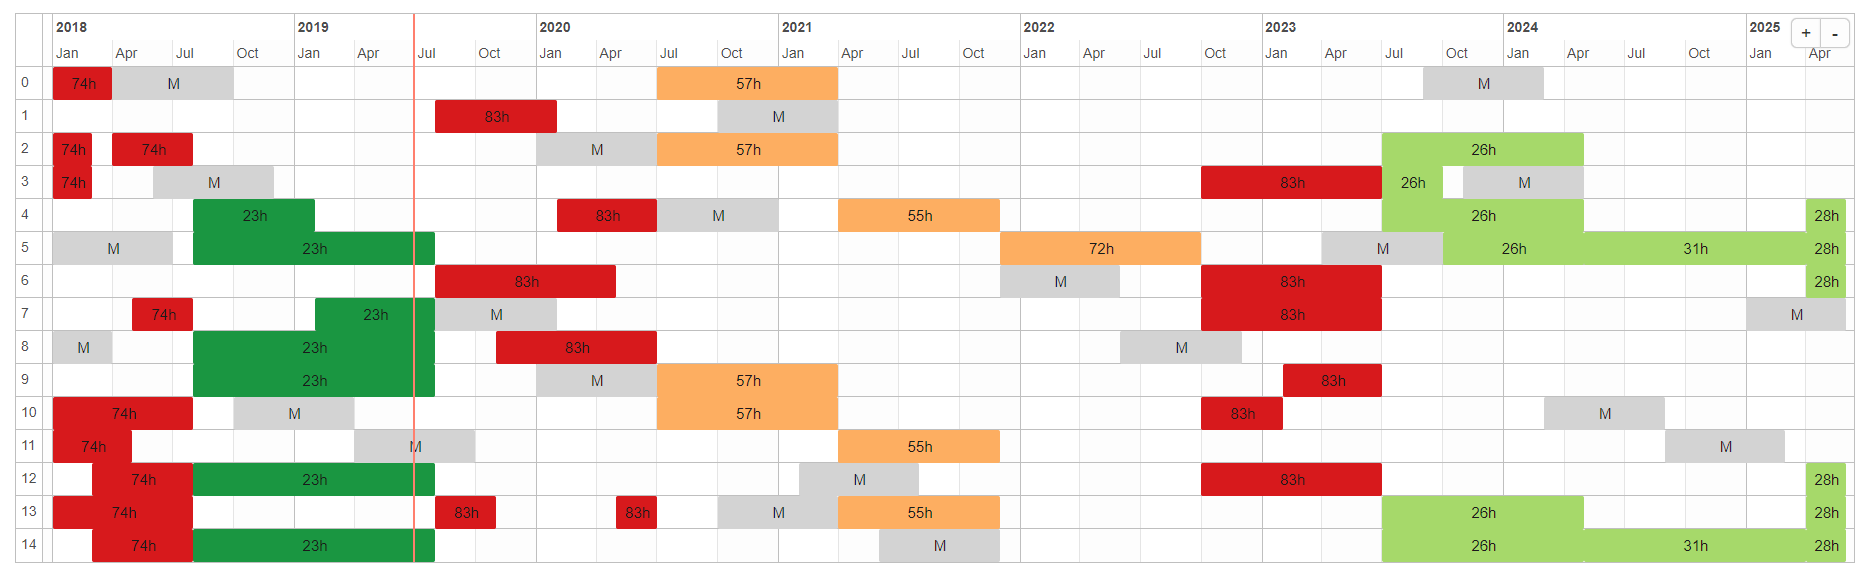
\includegraphics[width=0.7\linewidth]{calendar3}

\end{block}

\end{frame}

\begin{frame}

\begin{block}{Encoding of an MFMP solution}

\begin{align}
 a_{it} = 
  \begin{cases} 
   -1 & check \\
   0 & no\,\,assignment \\
   j & mission\,\, j \\
  \end{cases}\notag
\end{align}

Table format: a solution \(x\) is represented by a matrix
\(A = \mathbb{Z}^{I \times T}\).

Patterns: \(p \in \mathcal{P}\)

\(p = \{a_{i0}, a_{it}, a_{it+1}, ..., a_{iT}\}\)

Pattern format: a solution \(x\) is represented by a mapping
\(f: \mathcal{I} \to \mathcal{P}\).

\end{block}

\end{frame}
